\chapter{Tín hiệu âm thanh, tiếng nói. Thư viện PyAudio}
\ifpdf
    \graphicspath{{Chapter2/Chapter2Figs/PNG/}{Chapter2/Chapter2Figs/PDF/}{Chapter2/Chapter2Figs/}}
\else
    \graphicspath{{Chapter2/Chapter2Figs/EPS/}{Chapter2/Chapter2Figs/}}
\fi

\section{Tổng quan}
\subsection{Tổng quan về âm thanh}
Trong vật lý, âm thanh được định nghĩa là các giao động cơ học lan truyền thông qua các phương tiện truyền dẫn như: không khí, nước, chất rắn,... Các giao động cơ học đó còn được gọi là sóng âm. Sóng âm được tạo ra do có sự biến đổi về áp suất theo thời gian. Vận tốc lan truyền trong không khí của sóng âm vào khoảng 343.2 m/s.

Đối với con người, âm thanh là những giao động có thể được cảm nhận thông qua thính giác. Các giao động khi lan truyền trong không khí sẽ va đập và làm rung màng nhĩ, qua đó não bộ sẽ thu được tín hiệu âm thanh. Con người có thể nghe được âm thanh có tần số từ 16 Hz đến 20 kHz. Âm thanh có tần số cao hơn 20 kHz gọi là siêu âm, âm thanh có tần số thấp hơn 16 Hz gọi là hạ âm.

Cách đơn giản nhất để biểu diễn âm thanh là dưới dạng sóng sin với trục x là thời gian, trục y là áp xuất:

\begin{center}
$P = A\sin (2\pi ft)$
\end{center}

Trong đó: P là áp suất, đơn vị là decibels (dB) hoặc pascals \\
A là biên độ của sóng, đơn vị là decibels (dB) \\
t là thời gian, đơn vị là giây (s) \\
f là tần số, đơn vị là hertz (Hz)

\begin{figure}[h]
    \centering
    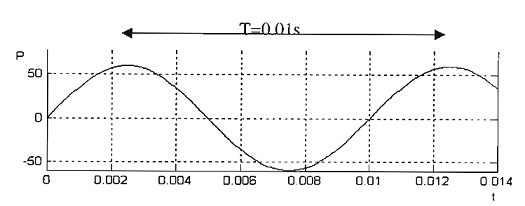
\includegraphics[scale=1]{sinwave}
    \caption{Sóng sin có biên độ 60 dB, tần số 100 Hz}
    \label{fig:c2_sinwave}
\end{figure}

Âm thanh có một số đặc trưng cơ bản như: độ cao, độ mạnh, độ dài và âm sắc.
\begin{itemize}
	\item \textbf{Độ cao} (Pitch): âm thanh luôn có một độ cao nhất định. Độ cao của âm thanh phụ thuộc vào tần số của sóng âm. Tần số càng lớn thì âm thanh càng cao, tần số càng bé thì âm thanh càng trầm.

	\begin{figure}[h]
		\centering
		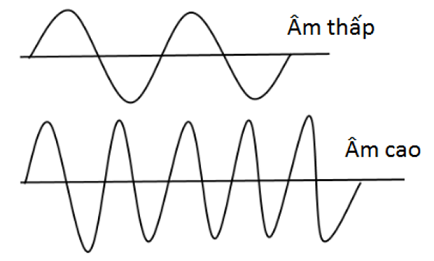
\includegraphics[scale=1]{pitch}
		\caption{Minh họa độ cao (Pitch) của âm}
		\label{fig:c2_pitch}
	\end{figure}

	\item \textbf{Độ mạnh} (Intensity): hay còn gọi là độ to của âm thanh. Độ mạnh của âm thanh phụ thuộc vào biên độ sóng âm. Biên độ càng lớn thi cường độ âm càng mạnh, biên độ càng bé thì cường độ âm càng yếu.
	\item \textbf{Độ dài} (Duration): là thời gian kéo dài của sóng âm.
	\item \textbf{Âm sắc} (Timbre): âm sắc là một đặc trưng sinh lý của âm, giúp phân biết âm thanh do các nguồn khác nhau phát ra. Âm sắc liên quan mật thiết với đồ thị giao động âm.
	\begin{figure}[h]
		\centering
		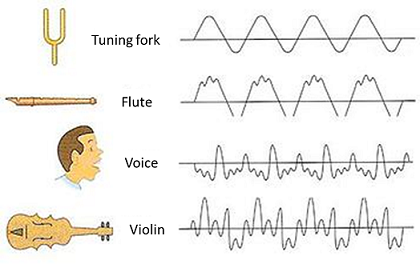
\includegraphics[scale=1]{timbre}
		\caption{Minh họa âm sắc (Timbre) của âm}
		\label{fig:c2_timbre}
	\end{figure}
\end{itemize}

Hiện nay âm thanh đã được nghiên cứu và ứng dụng rộng rãi trong nhiều lĩnh vực của cuộc sống như: truyền thông, âm nhạc, chế tạo sonar,...

\subsection{Tổng quan về tiếng nói}
Trong tự nhiên, âm thanh bao gồm nhiều loại được tạo ra từ nhiều nguồn khác nhau: 
\begin{itemize}
	\item \textbf{Âm nhạc}: âm thanh được phát ra từ các nhạc cụ.
	\item \textbf{Tiếng kêu}: được phát ra từ các loại động vật. Ví dụ: cá heo (1-164 kHz).
	\item \textbf{Tiếng động}: âm thanh phát ra từ sự va chạm giữa hai vật.
	\item \textbf{Tiếng ồn}: là những âm thanh không mong muốn.
	\item \textbf{Tiếng nói}: là những âm thanh được phát ra từ miệng con người
\end{itemize}

\noindent Ta có thể phân loại tiếng nói dựa theo thanh:
\begin{itemize}
	\item \textbf{Âm hữu thanh}: là âm khi phát ra có sự dao động của đôi dây thanh quản.
	\item \textbf{Âm vô thanh}: phát ra khi đôi dây thanh quản không dao động. Thí dụ phần cuối của phát âm English, chữ sh cho ra âm xát.
\end{itemize}

\noindent Hoặc theo âm:
\begin{itemize}
	\item \textbf{Nguyên âm}: là âm phát ra có thể kéo dài. Tất cả nguyên âm đều là âm hữu thanh, nghĩa là tuần hoàn và khá ổn định trong một đoạn thời gian vài chục ms.
	\item \textbf{Phụ âm}: là âm chỉ phát ra một nhát, không kéo dài được. Có phụ âm hữu thanh và phụ âm vô thanh.
\end{itemize}

Tiếng nói đóng vai trò quan trọng trong hoạt động động giao tiếp giữa con người, nó là phương tiện giao tiếp nhanh, tiện lợi và phổ biến nhất.

\section{Cách lưu trữ âm thanh trong máy tính}
Âm thanh trong tự nhiên có dạng liên tục 

Máy tính lưu trữ dạng rời rạc -> cần lấy mẫu âm thanh theo 1 tần số.
\subsection{Các thông số của âm thanh khi lưu trữ trên máy tính}
sample rate

bitdepth

chanel
...
\subsection{Lưu trữ không nén}
file wav
\subsection{Lưu trữ nén}
file mp3

\section{Ứng dụng}
Âm thanh là công cụ tương tác giữa người sử dụng và ứng dụng.

Người sử dụng sử dụng tiếng nói để ra lệnh

Ứng dụng dùng tiếng nói để phản hồi

\section{Thư viện PyAudio}
\subsection{Tổng quan}
Là thư viện viết bằng Python hỗ trợ tất cả các Hđh

Hỗ trợ người dùng tương tác với âm thanh trên máy tính dễ dàng.

https://people.csail.mit.edu/hubert/pyaudio/docs/
\subsection{Chức năng}
Thu âm từ microphone của máy tính dưới dạng dữ liệu thô

Phát âm thanh ra loa của máy tính từ dữ liệu thô
\subsection{Cài đặt}
pip

build từ source
\subsection{Cách sử dụng}
2 cách sử dụng: blocking, non-blocking

các thông số của ứng dụng: samplerate, bitdeptg, chanel, ...
\subsection{Các ưu, khuyết điểm}
Ưu: hỗ trợ nhiều hđh, cài đặt đơn giản, nhẹ, dễ sử dụng.
Nhược: ít tính năng, chưa hỗ trợ phát từ file mp3, chưa hỗ trợ thu từ nhiều micro
\subsection{Ứng dụng}
PyAudio được sử dụng trong module Microphone của ứng dụng. Giúp thu âm và chuyển cho các module khác để xử lý.





